\chapter{HTTP}
\label{cha:http}

\href{https://tools.ietf.org/html/rfc2616}{Request for Comments -
  RFC2616} is now replaced by the \uline{723x} series, of which
\href{https://tools.ietf.org/html/rfc7230}{RFC7230} is the
starting point, defining HTTP message and message routing.

\section{Glossary}
\label{sec:http-glossary}

HTTP was created for the World Wide Web (WWW) architecutre, and
much of the architecture is reflected in the terminology and
syntax defined in RFC723x series.

HTTP is a \textit{stateless} protocol that operates by exchanging
messages over \uline{transport-layer} or \uline{session-layer}
connection in a \textit{client-server} mode.

\textit{client} and \textit{server} refer to only the
\textit{role} that HTTP \textit{program}s perform for a
\textit{particular} connection. The same program might act as a
client on some connections or a server on others. A client
\textit{establish}es a connection for the purpose of sending one
or more \textit{request}s, a server instead \textit{accept}s
connections in order to serve requests by sending
\textit{response}s.

\textit{connection} means a transport-layer connection of TCP/IP
protocol stack between two endpoints. \textit{endpoint} is either
the client or server side of the connection. \textit{peer} is a
\textit{remote} endpoint. \textit{request} from client and
\textit{response} from server emphasize data transmission.

\textit{user agent} refers to any of the various \textit{client
  program}s on behalf of end users, including but not limited to
browsers (i.e. Firefox), spiders (web-based robots like
Googlebot), command-line tools (i.e. Curl), custom applications,
and mobile apps.

The term \textit{origin server} refers to the \textit{server
  program} that can \textit{originate} authorative responses for a
target resource.

An \textit{entity} is comprised of \textit{entity header}s and
\textit{entity body}. \textit{entity body} and \textit{payload}
both refer to the body part of a HTTP message like equation
\eqref{eq:message-body}. But entity emphasizes the data
representation of target resource while payload emphasizes syntax
of HTTP message.

\begin{equation}
  \label{eq:message-body}
  \begin{aligned}[t]
    \text{message-body} &= \text{Transfer-Encoding(entity-body)} \\
                        &= \text{Transfer-Encoding(Content-Encoding(Content-Type(target-resource)))}
  \end{aligned}
\end{equation}

\textit{target resource}, on the contrary, means the contents
stored on origin server. For each content, the server might have
multiple \textit{representation}s reflecting different versions of
the content, like modification date, compression etc. In other
words, a content may have multiple target resources that in turn
may have multiple entities.

HTTP supports the use of \textit{intermediaries} to satisfy
requests through \textit{a chain of connections}. There are three
common intermediaries: \textit{proxy}, \textit{gateway}, and
\textit{tunnel}. In some cases, a single intermediary might change
its type among proxy, gateway and tunnel based on the nature of
each request.

Terms \textit{upstream} and \textit{downstream} are used to
describe directional requirements in relation to \textit{message
  flow} regardless of requests or reponses: all messages flow from
upsteam to downstream. \textit{inbound} and \textit{outbound} are
used to describe directional requirements in relation to the
reponse: inbound means downstream response from the origin server
and outbound means downstream response to the user agent.

Proxy refers to \textit{forwarding proxy} and Gateway refers to
\textit{reverse proxy}. A proxy is a messsge-forwarding agent
selected by clients. A gateway acts as an origin server for
outbound connections but translates received requests to another
server, which is transparent to clients. Gateways are often used
to do CDN for performance improvement, load balancing across
multiple machines. Check the 502 (Bad Gateway) status code in
section \ref{sec:server-error-5xx}.

A proxy or gateway is defined in the context of HTTP
communication. There are also proxies that can act on
\textit{lower} layers of the network protocol stack, filtering or
redirecting HTTP traffic without the knowledge or permssion of
HTTP participants. For example, \textit{interception proxy} (also
commonly known as \textit{transparent proxy}) is selected by
neither client nor server sides.

A tunnel is just a \textit{blind relay} between two connections
without changing the messages. Once active, a tunnel is not
considered a party to the HTTP communication. The tunnel is not
aware of any HTTP syntax or semantics.

Before ending this section, let's recall the term stateless. This
term means each request can be understood or parsed standalone,
withou any prior knowledge. A server MUST NOT assume that two
requests on the same connection are from the same user
agent. Specially, the ``stateless'' feature enables reuse of
\textit{cache}, and load balancing across multiple servers.

\section{Cache}
\label{sec:http-cache}

A cache is a local store of previous response messages and
a relevant subsystem that controls its storage, retrieval, and
deletion.

The purpose of a cache is to store \textit{cacheable} responses in
order to reduce the \textit{response time} and network
\textit{bandwidth consumption} on future, equivalent
requests. Please pay attention, not all reponses are cacheable
such as that of POST and PUT (read more in section
\ref{sec:put-post}.

The effect of a cache is that the request/response chain is
shortened if one of the intermediaries along the chain has a
cached response applicable to that request like figure
\ref{fig:shortened-http-chain}.

\begin{figure}[bp]
  \centering
  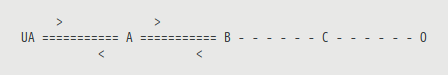
\includegraphics[scale=0.5]{shortened-http-chain}
  \caption{Shortened HTTP Chain}
  \label{fig:shortened-http-chain}
\end{figure}

\subsection{URL URI}
\label{sec:url-uri}

URI is the superset of URL in general. However, within an URL, the
part after the domain name (including the leading forwardslash) is
also a type of URI which, in RFC, is called \textit{resource
  identifier}.

\href{https://stackoverflow.com/q/28592077}{Regarding Nginx},
vairable \verb|request_uri| is the equivalent of URI while
variable \verb|uri| is the normalized \verb|request_uri| without
query string.

\section{HTTP Method}
\label{sec:http-method}

\subsection{PUT POST}
\label{sec:put-post}

\href{https://stackoverflow.com/a/630475}{POST and PUT} both can
be used for \textit{creating} and \textit{updating} resources on
servers.

PUT sends an entity with a specified URI location to the
server. If there already exists an entity on that URI, it will be
updated (replaced by the new one). Otherwise, the new entity is
created (put) on the server. So we know that the PUT method
requires an given URI identifier in the request.

PUT is \textit{idempotent} (幂等) similar to variable assignment
like \verb|x = 5|. If an entity are put multiple times, it makes
no difference and the result is guaranteed.

POST is almost the same as PUT but cannot be used to to create a
new entity on a given URI. That is to say, the identifier part of
an URI when creating is determined by the server side
semantics. For example, this request would probably receive a 4xx
status code (probably 404) when creating a new question to
\textit{stackoverflow.com}:

\begin{lstlisting}
POST /questions/http-put-vs-post HTTP/1.1
Host: stackoverflow.com
\end{lstlisting}

Instead, please remove the resource identifier:

\begin{lstlisting}
POST /questions/ HTTP/1.1
Host: stackoverflow.com
\end{lstlisting}

The server will create the resource identifier on
demand. Therefore, POST creates a \textit{subsidiary}
resource. Here is an excerpt from the Internet:

\begin{quotation}
  From the other side of the fence: PUT if the client determines
  the resulting resource's address, POST if the server does it.
\end{quotation}

Apparently, POST is \textit{not idempotent} when \textit{creating}
the same entity multiple times as the identity part is not
controlled by the client side, resulting in duplicate entities
located under different URIs.

As both PUT and POST create or update entities, reponses are
\textit{not} cacheable as those operations are expected to execute
\textit{only once} by nature. If a PUT or POST request was cached,
then cache servers (including user agents) would repeat the
request unintentionally and the relevant entity would be created
or updated repeatedly too. To the contrary, a GET method only
reads entity from servers and can be cached.

\subsection{GET POST}
\label{sec:get-post}

The advantage of GET over POST is that everything about a GET
request is stored in the URI. So it is quite easy to be
manipulated on the fly; recorded by search engine; bookmarked by
browser; cached by proxy etc.

In terms of method security, POST is advantageous over GET. When
GET something from the server, the request URI can be tracked
through browser history, server log and search engine
(i.e. Google) . On the other hand, desired action of POST method
is embedded in the message body and cannot be cached. However,
both methods use plain text transfer and can sniffed easily unless
HTTPS is adopted.

\section{HTTP Response Status Code}
\label{sec:http-response-status-code}

In this section, \textit{response code}, \textit{status code}, and
\textit{response status code} are referred to interchangeably, and
mean almost the same thing: an three-digit integer from web server
indicating the request and reponse status. The name
\textit{response} represents the HTTP reply message.

\begin{figure}[tbp]
  \centering
  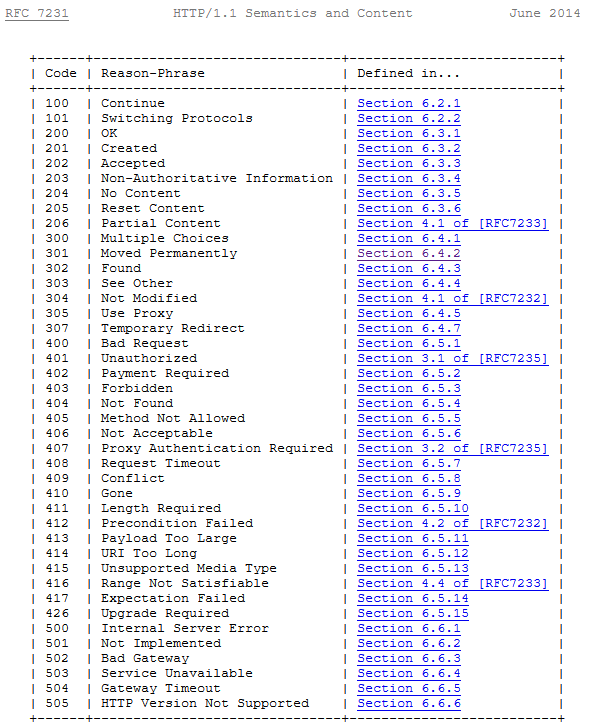
\includegraphics[width=.60\textwidth]{http-status-code}
  \caption{HTTP Status Code}
  \label{fig:http-status-code}
\end{figure}

For authorative reference, check
\href{https://tools.ietf.org/html/rfc7231/rfc7231}{RFC7231}. Figure
\ref{fig:http-status-code} defines the list of available official
codes. They are grouped into five categories, with the first digit
defining the code class:

\begin{itemize}
\item 1xx \textit{informational response}: the request was
  received, continuing process.
\item 2xx \textit{successful response}: the request was
  successfully received, understood, and accepted.
\item 3xx \textit{redirect}: futher action needs to be taken in
  order to complete the request.
\item 4xx \textit{client error}: the request contains bad syntax
  or cannot be fulfilled.
\item 5xx \textit{server error}: the server failed to fulfill an
  apparently valid request.
\end{itemize}

HTTP clients are not required to understand all registered status
codes, though such understanding is obviously desirable. However,
a client MUST understand the class (namely, the first digit) of
any received code, and treat an unrecognized status code as being
equivalent to the x00 status code of the x class where x belongs
to ${1,2,3,4,5}$, with the exception that a \textit{recipient}
(i.e. proxy server) MUST NOT cache a response with an unrecognized
status code.

Responses with status codes (by default, 200, 203, 204, 206, 300,
301, 400, 404, 410, 414, and 501) can be cached for hueristic
expiration unless otherwise indicated the method definition or
explicit cache
controls. \href{https://tools.ietf.org/html/rfc7234}{RFC7234}
defines HTTP caches and the associated header fields that control
cache behavior or indicate cacheable response messages.

\subsection{Informational 1xx}
\label{sec:informational-1xx}

The 1xx class of status code indicates an \textit{interim}
response for communicating connection status or request progress
\textit{prior} to completing the requested action and sending a
final response.

The 100 (Contine) status code indicates that the initial part of a
request has been received and has not yet been rejected by the
server. The server intends to send a final response after the
request has been fully reeived and acted upon.

The 101 (Switching Protocols) status code indicates that server is
willing to change application protocol like upgrading to a newer
HTTP version.

\subsection{Successful 2xx}
\label{sec:successful-2xx}

The 2xx class of status code is mostly desired, indicating the
request was successfully received, understood, and accepted.

Of the 2xx class, the 200 (OK) status code is what a client
expects largely and always (except the CONNECT method) has a
payload, though an origin server MAY generate a payload body of
zero length.

The 201 (Created) status code indicates that the request has been
fulfilled and one or more new resources have been created (PUT,
POST etc. methods).

The 202 (Accepted) status code indicates that the request has been
accpeted for processing, but the processing has not been
completed.

The 203 (Non-Authoritative Information) status code indicates that
the request was successful but the enclosed payload has been
modified by a transforming proxy. For example, image format is
changed in an intermediate web proxy.

The 204 (No Content) status code indicates that the server has
successfully fulfilled the request and that there is no additional
content to send in the response payload body (PUT, POST
etc. methods). Action is successfully applied to the server and
the user agent will inform its user the success (i.e. a dialog pop
up).

\href{https://tools.ietf.org/html/rfc7233}{The 206 (Partial
  Content)} code means the server is successfully fulfilling a
range request for the target resource by transferring one or more
parts of the selected representation that corresponds to the
satisfiable ranges found in the request's Range header field.

\subsection{Redirection 3xx}
\label{sec:redirection-3xx}

The 3xx (Redirection) class of status code indicates that further
action needs to be taken by the user agent in order to fulfill the
request. Most of the time, the user agent will send another
reqeust to the new URI specified in Location header field in the
response.

User agents diverge on the method applied to the second
request. In HTTP 1.0, 301 (Moved Permanently) and 302 (Found) are
defined to use the same method as the original reqeust, while 303
(See Other) rewrites method as GET regardless of the original
method. However, most user agent implementations always rewrite
the method as GET despite 301, 302 or 303.

Considering the implementation prevalence, HTTP/1.1 \textit{has
  to} acknowledge the de facto practice, and added 307 (Temporary
Redirect) and 308 (Permanent Redirect) to \textit{explicitly}
disallow method rewrite. In other words, original POST method
cannot be rewritten to GET. Table
\ref{tab:redirect-and-method-rewrite} is a summary of method
rewrite from \href{https://tools.ietf.org/html/rfc7231}{RFC7231}
and \href{https://tools.ietf.org/html/rfc7238}{RFC7238}.

\begin{table}[tbp]
  \centering
  \begin{tabular}[tbp]{c|c|c}
    \toprule{}
    Method & Permanent & Temporary \\
    \midrule{}
    POST to GET & 301 & 302 \\
    POST & 308 & 307 \\
    GET & & 303 \\
    \bottomrule
  \end{tabular}
  \caption{Redirect and Method Rewrite}
  \label{tab:redirect-and-method-rewrite}
\end{table}

Permanent redirect means future requests of the target resource
should be sent to the new URI while temporary redirect sticks to
the old URI. When upgrading HTTP to HTTPS or switching
\textit{php} to \textit{html}, 301 permanent redirect can be
adopted. The 302 status code can be classified into
\textit{on-domain} redirect (same domain name) and
\textit{off-domain} redirect (different domain name). For example,
users are usually redirected to a login URI temporary. Regardless
of 301 or 302, domain name redirect is discouraged, which requires
proper design at the very beginning of service deployment.

The 303 (See other) redirect explicitly rewrites request method as
GET/HEAD to \textit{retrieve} the target resource, and does not
imply permanent or temporary redirect. Name ``retrieve'' is chosen
as the new URI in the response is intended to provide only
\textit{descriptive} information on the final
target. Consequently, 302 redirect is also called \textit{indirect
  redirection} as further redirections may be required.

The redirect difference between 301 and 302 make a difference when
Search Engine Optimization (SEO) is concerned. If domain name
change is done with 301 redirect, then the Page Ranking (PR) of
the old domain name is probably lost. When a 302 redirect is
encountered, search engine by default attributes the page ranking
to the original URI. Search engines may downgrade the PR as a
target resource is preferred to be located by an unique URI.

Specially, 302 redirect is utilized to do
\href{https://en.ryte.com/wiki/URL_Hijacking}{URL Hijacking},
basically, stealing PR of another domain for the favor of
hijackers' page contents. At the very beginning, a hijacker should
find a way to achieve 302 redirect. For example, hack the target
web server and embed a 302 directive directly in the HTML file or
through Nginx \textit{rewrite} directive. Other methods are like
\href{https://blog.csdn.net/mgxcool/article/details/47206835}{DNS
  Hijacking},
\href{http://xsk.tehon.org/den/index.php/category/tech/tcp-bypass-hijacking-feature-and-recognization.html}{Bypass
  Interception} etc. When a user searches keywords covered in the
hijacker's page, search engine would probably return the original
URL that would be then redirected to the hijacker's URL. Once
succeeded, the PR of the original page is contributed to the
hijacker's page.

Another interesting code is 304 (Not Modified). This code is
returned when a conditional GET or HEAD request is received but
the condition is evaluated to false. In other words, the target is
not modified and the user agent has a up-to-date representation of
the target resource. There is no need to transfer another
representation of the target resource. Therefore, the 304 response
\textit{must not} contain a message-body.

More details,
please check section \ref{sec:last-modified}.

\subsection{Client Error 4xx}
\label{sec:client-error-4xx}

The 4xx class indicates the client seems to have erred. The 400
(Bad Reqeust) status code means the server cannot fulfill the request due to
malformed request syntax, invalid URI, deceptive request routing
etc.

401 (Unauthorized) indicates that the request has not been applied
because it lacks valid authentication credentials for the target
resource. 403 (Forbidden) indicates that the server understands
the request but refuses to authorize it like invalid credentials.

404 (Not Found) indicates the server cannot find a
current representation for the target resource or is not willing
to disclose existence.

410 (Gone) indicates access to the target resource is no longer
available (i.e. removed) at the origin server. It is common for
limited-time, promotional services and for resources belonging to
individuals no longer associated with the origin server's site.

405 (Method Not Allowed) indicates that the method recevied in the
request-line is known by the origin server but not supported by
the target resource.

416 (Range Not Satisfiable) indicates none of the ranges in the
request's Range header field \textit{overlap} the current extent
of the selected resource.

\subsection{Server Error 5xx}
\label{sec:server-error-5xx}

The 5xx (Server Error) class indicates that the server is aware
that it has erred or is incapable of performing the requested
method. The 500 (Internal Server Error) code indicates the server
encountered an unexpected condition that prevented it from
fulfilling the request. The 501 (Not Implemented) code means the
server does not support the functionality required to fulfill the
request.

The 502 (Bad Gateway) status code means the server, while acting
as a proxy or gateway, received an invalid response from an
inbound (upstream direction) server it accessed while attempting
to fulfill the request. The 504 (Gateway Timeout) code indicates
that the server, while acting as a gateway or proxy, did not
receive a timely response from an upstream server it needed to
access in order to complete the request.

The 503 (Server Unavailable) indicates the server is currently
unable to handle the request due to temporary overload or
scheduled maintenance. The situation might be allievated after
some delay.

\section{Headers}
\label{sec:http-headers}

\subsection{Last-Modified}
\label{sec:last-modified}

\uline{Last-Modified} is a reponse header field providing a
timestamp indicating the date and time at which the origin server
believes the selected representation was last modified.

\uline{If-Modified-Since} is a request header field, making the
entity transfer conditional on the modification date of remote
version being more recent than the field value.

When a cache party is involved, it will typically use the value of
the cached message's Last-Modified field to generate
If-Modified-Since. However, occasionally, other source data might
be used such as the \uline{Date} header field of the cached
message.

The combination of Last-Modified and If-Modified-Since limits the
scope of a web traversal to resources that have recently changed
and reduce bandwidth.

\subsection{ETag}
\label{sec:etag}

\uline{ETag} is another response header field providing the
current \textit{entity tag} for the selected representation, as
determined at the conclusion of handling the request. It is an
opaque string (i.e. a MD5 hash) differentiating between multiple
representations of the same entity.

Similar to the Last-Modified and If-Modified-Since pair, a client
can also use ETag values using If-Match or If-None-Match (analyzed
below) to do conditional requests and may save bandwidth and
response time. However, ETag is more reliable than date value when
it is inconvenient to store modification dates or when date values
is not accurate due to clock synchronization

The preferred behavior for an origin server is to send both a
strong entity-tag and a Last-Modified value in successful
responses to a retrieval request.

\subsection{If-None-Match}
\label{sec:if-none-match}

The \uline{If-None-Match} header field makes the request method
conditional on a recipient cache or origin server either not
having any current representation of the target resource when the
field value is '*', or having a selected representation with an
entity-tag that does not match any of those listed in the field
value.

Most of the time, the field value is set to be a list of cached
entity-tags. The server only responses a representation of which
the entity-tag does not appear in the list.

The special asterisk can prevent unsafe methods (i.e. PUT and
POST) from creating or updating a target representation multiple
times, resulting in ``lost update'' issue as any entity-tag on the
server will match the wildcard '*'.

On the other hand, there is the \uline{If-Match} header field in a
request. Upon receiving such requests, the server only performs
the method when the representation entity-tage match any of the
field value. If the value is wildcard '*', it requires at least
one representation exist.

Table \ref{tab:condi-hed-cache-vld} shows the combination of
conditional headers.

\begin{table}[tbp]
  \centering
  \begin{tabular}[tbp]{r|l}
    \toprule
    Request Header & Reponse Header \\
    \midrule         
    If-Match & Etag \\
    If-None-Match & Etag \\
    If-Modified-Since & Last-Modified \\
    \bottomrule
  \end{tabular}
  \caption{Conditional Header and Cache Valiador}
  \label{tab:condi-hed-cache-vld}
\end{table}

\subsection{Forwarded}
\label{sec:http-forwarded}

\uline{Forwarded} is an \textit{extended} and \textit{optional}
HTTP \textit{header field} that, when used, contains a list of
\uline{parameter:identifier} pairs that disclose information
\uline{for} the \textit{client}, about the \uline{host} header
field and/or the \uline{proto}, or \uline{by} \textit{proxies}
when one or more proxies are involved in the chain of
\textit{request} connections

This header field is only used for HTTP requests and is not to be
used in HTTP responses. Due to the sensitive nature of disclosed
information, this header field should be turned off by
default. Further, it applies to reverse proxies, as well as
forwarding proxies. The following are samples added by a proxy:

\begin{lstlisting}
Forwarded: for="_gazonk"
Forwarded: For="[2001:db8:cafe::17]:4711"
Forwarded: for=192.0.2.60;proto=http;by=203.0.113.43
\end{lstlisting}

The identifier is a
\href{https://tools.ietf.org/html/rfc7239#section-6.3}{Obfuscated
  Identifier} that keep the IP address secret, while still
allowing the ``Forwarded'' header field to be used for tracing and
debugging.

From
\href{https://tools.ietf.org/html/rfc7230#section-3.2}{RFC7230}, a
\textit{header field} consists of a \textit{case-insensitive}
field name followed by a colon (\uline{:}), optional leading
whitespace, the field value and optional trailing whitespace. The
field name ``Forwarded'' can be written as lower case
``forwarded''. Pay attention please, \textit{parameter}s in the
field value are also case-insensitive. So ``for'' and ``For'' are
equivalent.

Pairs should be semicolon-separated within the field value
part. Each parameter must not occur more than once per field
value. In other words, an individual proxy can add only one
instance of a particular parameter.

A subsequent proxy that wants to add a new field value can either
append it to the last field value after a \textit{comma
  separator}, or add another ``Forwarded'' header field. Here is
an example:

\begin{lstlisting}
Forwarded: for=192.0.2.43, for=198.51.100.17
\end{lstlisting}

The two \uline{for} pairs are separated by a comma, representing
two field values added different proxies in the request chain.

For the list of field values, the very first field value is added
by the very first proxy, and each subsequent field value is
appended by each subsequent proxy. The \uline{for} parameter for
the last proxy in the chain is not required, as the upstream
server get its IP from the TCP connection directly.

A proxy can add a set of \uline{parameter:identifier} pairs; it
can also remove existing pairs added by previous proxies. Because
this header field is optional, any proxy in the chain may choose
not to update this header field. Please read more details from
\href{https://tools.ietf.org/html/rfc7239}{RFC7239}.

However, in reality, the ``Forwarded'' header field name is
implemented as \textit{X-Forwarded-For}. Nginx has two relevant
built-in variables to record the field value, namely
\lstinline|$proxy_add_x_forwarded_for| and
\lstinline|$http_x_forwarded_for|. The syntax is a bit different
from what is specified in the RFC. Here is a common setting on a
reverse proxy:

\begin{lstlisting}
proxy_set_header            X-Forwarded-For $proxy_add_x_forwarded_for;
\end{lstlisting}

Both variables may or may not be related to another built-in
variable \lstinline|$remote_addr| which is the IP address of the
preceding origin in the chain, derived from the underlying TCP
connection. Basically,
\lstinline|$proxy_add_x_forwarded_for| will \textit{append}
\lstinline|$remote_addr| to
\lstinline|$http_x_forwarded_for| that is the received field value
of ``X-Forwarded-For'' from the preceding origin in the chain. If
the Nginx is the very first proxy, then
\lstinline|$http_x_forwarded_for| would be empty.

By the way, the field value of ``X-Forwarded-For'' can be forged
easily by manipulating the request header:

\begin{lstlisting}
curl http://www.example.com -H 'X-Forwarded-For: a.b.c.d' -H 'X-Real-IP: e.f.g.h'
\end{lstlisting}

Often, the ``X-Forwarded-For'' is accompanied by another optional
field \uline{X-Real-IP} that records the
\lstinline|$remote_addr| like:

\begin{lstlisting}
proxy_set_header            X-REAL-IP $remote_addr;
\end{lstlisting}

Unlike the \textit{add} or \textit{append} nature of
\lstinline|$proxy_add_x_forwarded_for|, \uline{X-REAL-IP} is
always overwriten by the current proxy. So it cannot be forged by
manipulating the request header.

\section{CORS}
\label{sec:cors}

The \textit{name} \uline{origin} refers to a \textit{tuple}
consisting of \textit{protocol}, \textit{domain} and
\textit{port}:

\begin{lstlisting}
(protocol, domain, port)
\end{lstlisting}

It is a property derived from web URL. Any variation of the three
values denotes a different origin. Two URLs have the \textit{same
  origin} if the protocol, domain, and port (if specified) are the
same for both. The two URLs below have different origin as the
ports are different.

\begin{lstlisting}
http://www.example.com/data/cat.jpg
https://www.example.com/data/cat.jpg
\end{lstlisting}

Script (i.e. JS) URLs in the form of \textit{about:blank} or
\textit{javascript:} do not define a origin as protocol, domain,
and port are \textit{all absent}. Such script \textit{inherit}s
the origin of the document containing the URL.

Before telling about what Cross-Origin Resource Sharing (CORS) is,
let's have a look at
\href{https://developer.mozilla.org/en-US/docs/Web/Security/Same-origin_policy}{same-origin
  policy}. It is a critical mechanism that restricts how a
document or script loaded from one origin can interact with a
resource from another origin.

We call interactions between different origins
\textit{cross-origin} access, such as when we use
\href{https://developer.mozilla.org/en-US/docs/Web/API/XMLHttpRequest}{XMLHttpRequest}. It
is a rule enforced by web browsers, not that of web servers. By
default, a web browser does not allow cross-origin HTTP requests,
where
\href{https://developer.mozilla.org/en-US/docs/Web/HTTP/CORS}{CORS}
comes into being. Figure \ref{fig:cors} gives a clear
illustration.

Loading the script file itself does \textbf{not} belong to
cross-origin access and is not restricted by the same-origin
policy. It is what the script executes after loading that do
cross-origin access.

\begin{figure}[!htb]
  \centering
  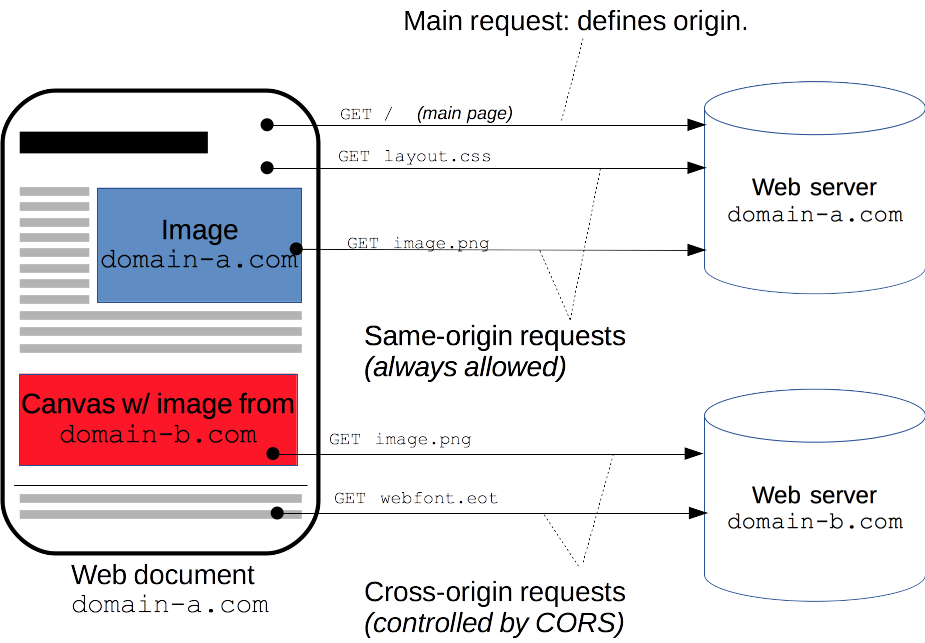
\includegraphics[width=.8\textwidth]{CORS_principle}
  \caption{Cross-Origin Resource Sharing}
  \label{fig:cors}
\end{figure}

CORS refers to Cross-Origin Resource Sharing, letting a web server
specify whether other web servers are permitted to load content
from it. It uses additional HTTP headers to tell a
\textit{browser} that a web application for one \textit{origin}
has permission to access selected resources from another web
application for a \textit{different origin}.

A web application should executes \uline{cross-origin HTTP
  request} when it requests a resource served by a different
origin than its own. Such requests cotain a HTTP header named as
\uline{Origin}. For example, the frontend Javascript code for a
web application served under the origin of
\uline{http://domain-a.com} uses XMLHttpRequest to make a request
for data \uline{http://api.domain-b.com/data.json}. The request
headers include \uline{Origin: http://domain-a.com} which
manifests how the term ``origin'' comes into being.

Whether the response is blocked or not by the broswer depends on
response header \uline{Access-Control-Allow-Origin}, indicating
whether the response can be shared with requesting code from the
given origin like:

\begin{lstlisting}
Access-Control-Allow-Origin: *
Access-Control-Allow-Origin: http://api.domain-b.com
Access-Control-Allow-Origin: null
\end{lstlisting}

The special wildcard \verb|*| means to allow CORS from any
origin. Apart from the simple XMLHttpRequest, CORS also supports
other methods like
\href{https://developer.mozilla.org/en-US/docs/Web/HTTP/CORS#Preflighted_requests}{Preflighted
  Request}. CORS is only one of the mechanisms to achieve
cross-origin access. There exists
\href{https://stackoverflow.com/q/2067472}{JSONP} to execute the
same will. However JSONP is almost outdated and you only require
it for older browsers.

简单用中文说:

\begin{itemize}
\item The Same-Origin Policy 叫同源策略。在没有同源策略之前,浏览器
  里不同源的代码和内容可以随意交互,不受限制。这会带来安全隐患,
  如 Origin A 的恶意代码可以访问 Origin B 上的安全信息。
\item 完全遵守同源测策也使 HTTP 应用灵活性降低。如同一 Origin 里的
  域名可以有很多别名 CNAME, 因此诞生了跨域(跨源)访问机制。其中一
  种就是本文讲的 CORS. 简单来讲,就是服务器端告诉浏览器,哪
  些Origin 可以对本 Origin 进行跨域访问。
\item Origin A 服务器上的 js 脚本以 CORS 方式抓取 origin B 服务器上
  的内容,浏览器会检查 B 的响应
  头 \text{Access-Control-Allow-Origin}, 如果响应头中包含 origin A
  则显示返回的内容,否则禁止。
\item Origin A 从 Origin C 加载 JS 脚本这个行为本身不属于跨域范筹,
  不受同源测策略限制。脚本在加载完毕后,对 Origin B 执行的请求才是
  跨域访问。
\item 跨域只存在于浏览器端,不存在
  于 android/ios/Node.js/python/java 等其它环境。跨域请求能发出去,
  服务端能收到请求并正常返回数据,只是结果可能被浏览器拦截了。如果
  需要禁止对服务器的访问,则需要上“防盗链”或“鉴权”。
\end{itemize}

\section{Websocket}
\label{sec:websocket}

The \href{https://tools.ietf.org/html/rfc6455}{websocket} protocol
is a different protocol from HTTP for its own purpose, though they
are related. Basically they are at the same layer over protocol
stack and both sit on top of TCP connection.

Websocket is created not to replace HTTP but to meet new web
requirements like \textit{high throughput} and \textit{low
  latency}. In order to be compatible with existing web
infrastructure, Websocket makes use of HTTP handshake by the
header fields \uline{Upgrade: websocket} and \uline{Connection:
  Upgrade} at port 80 or 443. Upon receving the HTTP handshake
request, the websocket server responds with status code 101
(Switching Protocols). From then on, the protocol is switched from
HTTP to websocket. All following transmission is carried over the
TCP connection just established. Like HTTP, it is a
\textit{message} protocol with each message 6 bytes
headers. However, 6 bytes is negligible compared to HTTP headers.

At the very beginning, Websocket is one of the features
(i.e. \uline{Local Storage} and \uline{Geolocation}) defined by
the \href{https://en.wikipedia.org/wiki/HTML5}{HTML5}
specification and is now moved to a standalone protocol to keep
the subjet focused. Hence, it is not unusual to call it
\uline{HTML5 Websocket}.

Next I will talk about the purpose of Websocket and why it is
invented alongside with HTTP. HTTP requires
\textit{synchronization} with strict \textit{request} and
\textit{response} pair order. only the \textit{client} side can
initiate the communication while the \textit{server} side
cannot. We call it a \uline{request/response protocol}.

A HTTP/1.0 TCP connection allows only one request sent out at any
given moment on a given TCP connection. After getting the
response, the TCP connection would be closed and the client can
send out a new request. However, a new TCP connection needs
created. Such a synchronized request and response method brings in
extra bandwidth and increases latency.

That is changed in HTTP/1.1 where the
\href{https://tools.ietf.org/html/rfc6223}{keep-alive} feature
keeps the underlying TCP connection open for further request and
response pairs. Therefore, it is also called
\href{https://en.wikipedia.org/wiki/HTTP_persistent_connection}{HTTP
  Persistent Connection}. Another feature of HTTP/1.1 is
\uline{HTTP pipeline}. Based on persistent connection, The client
do not have to wait for responses before sending out new
requests. So requests can sent out in line in series. However, the
responses must arrive in
\href{https://stackoverflow.com/a/34479053}{the exact order} as
requests. Therefore, it is not a true multiplexing method. Most
existing infrastructure (including Chrome/Firefox) disables HTTP
pipeline by default.

HTTP/1.1 introduces
\href{https://tools.ietf.org/html/rfc7230#section-3.3.1}{Transfer-Encoding}
mechanism, an interface towards the TCP socket. It us not unusual
we call it \uline{HTTP Streaming} as Transfer Encoding allows
sending of a resource representation in a set of \uline{chunk}s
sequentially. Chunks are sent and recived from the persistent TCP
socket. It is HTTP application's role to reassemble the
chunks. Upon receving all the chunks, the client reassembles them
as a whole - the response! Transfer-Encoding fits dynamically
generated content.

However, the \uline{request/response model} still cannot satisfy
modern real-time transmission requirements. The request and
response headers are still present but most of them are almost
identical - \textit{redundant} data. Also, the pipeline by nature
demands strict order! That is to say, the synchronization feature
is still present, which suffers from
\href{https://stackoverflow.com/q/45583861}{Head-of-Line (HOL}
blocking. If the very first request of the pipeline is somehow not
delivered as fast as expected, the requests behind are all
blocked!  Accordingly, clients (also applies to HTTP/1.0) need to
make many requests use multiple connections to a server in order
to achieve concurrency and thereby reduce latency.

On the other hand, Websocket is a \textit{asynchronous
  full-duplex} protocol designated for \textit{high throughput}
and \textit{low latency}. Firstly, it is a full-duplex
protocol. Once the TCP connection is established, it is ready for
data transmission from and to either side, regardless of client or
server, namely \textit{server push}. HTTP may utilize
\href{https://stackoverflow.com/q/12555043}{polling or long
  polling} (somehow a stupid workaround) or \textit{plugin}s like
\uline{Java Applet}, \uline{Flash}, and
\uline{Silverlight}. However, a plugin may not be accepted by
intermediaries (CDN, proxies or firewalls), require cusotom ports,
and is subject to security vulnerabilities. Websocket reuses
well-known port 80 or 443 to be compatible with exsiting web
deployment. When a firewall or proxy intermediate party is
detected, Websocket automatically sets up a tunnel to pass through
by issuing a HTTP \uline{CONNECT} method.

As you see, data is sent out on demand, which is also called
\textit{server push}. Once data is ready, it is pushed to the
client immediately. The asynchronization nature increases
throughput greatly as the request/response synchronization hazard
is relieved. Both sides can send data simultaneously. Figure
\ref{fig:websocket-vs-http} illustrates the transmission schemes
between Websocket and HTTP.

\begin{figure}[!htb]
  \centering
  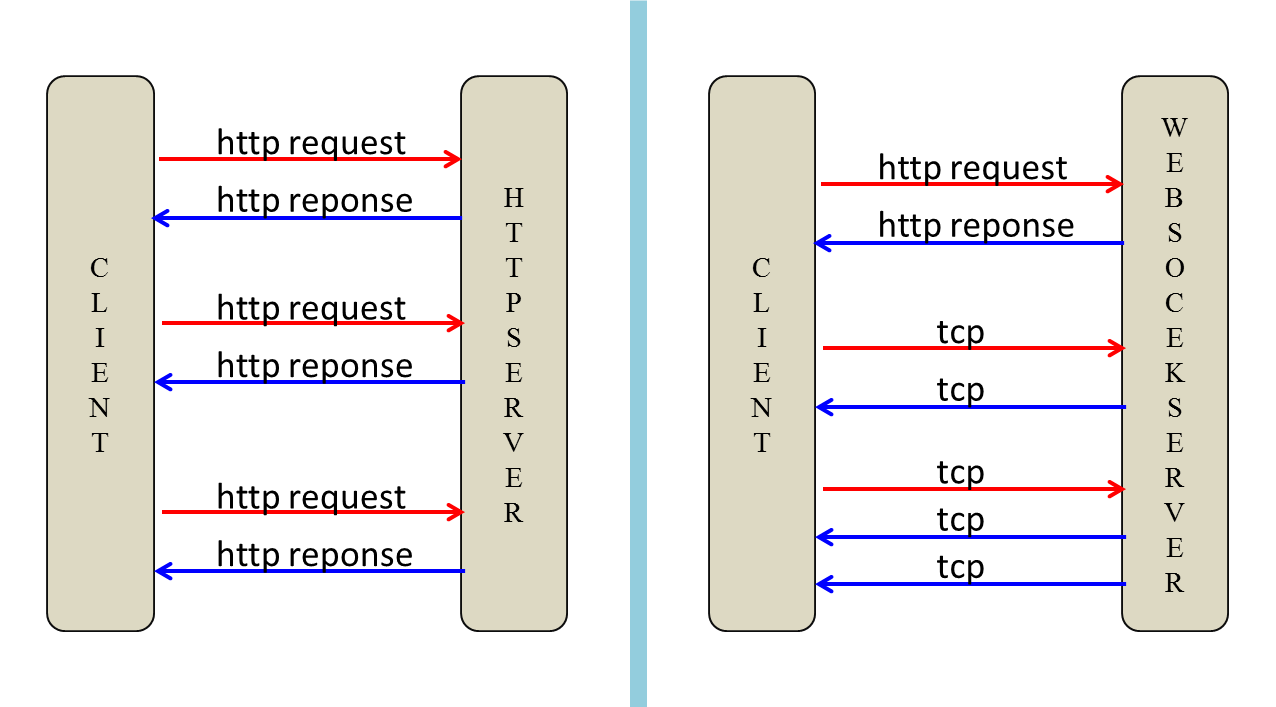
\includegraphics[scale=.5]{compareWebsocketHttp}
  \caption{Websocket vs HTTP}
  \label{fig:websocket-vs-http}
\end{figure}

With high throughput and low latency, Websocket fits application
like video games, stock trending, customer support, live streaming
etc. Whereas, HTTP has its own vantage points. It is much simpler
and has a well-supported ecosystem. Unless required, please resort
to HTTP first. Aslo, they can be combined together in live
streaming like \uline{HTTP+Websocket+FLV}. Figure
\ref{fig:live-streaming} shows the data flow of existing live
streaming applications.

\begin{figure}[!htb]
  \centering
  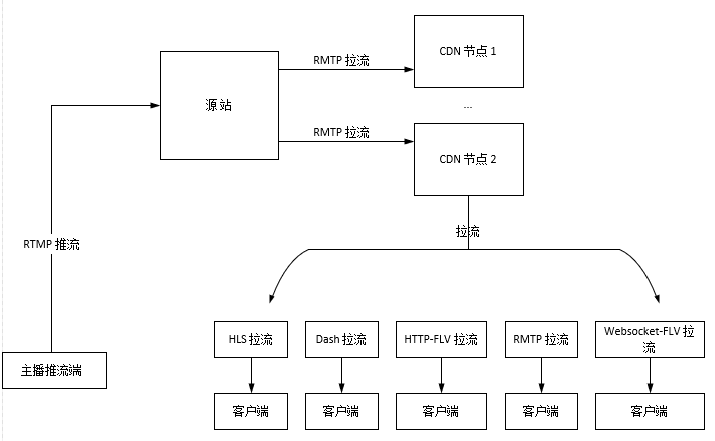
\includegraphics[scale=.5]{livestreaming}
  \caption{Live Streaming}
  \label{fig:live-streaming}
\end{figure}

To understand Websocket better, read
\href{http://www.importnew.com/28036.html}{再谈 Websocket 架构设计}
and \href{http://www.websocket.org/aboutwebsocket.html}{About
  Websocket}.

\section{HTTP/2}
\label{sec:http2}

In section \ref{sec:websocket}, we discussed the difference
between HTTP/1.0, HTTP/1.1 and Websocket. Websocket is an ideal
alternative to HTTP when serving applications of high throughput
and low latency like live streaming. However, it is \textit{less
  supported} by real world infrastructure compared with HTTP. That
is how HTTP/2 (not 2.0) comes into being. The name \uline{h2}
identifies the protocol where HTTP/2 over TLS while \uline{h2c}
identifies HTTP/2 over cleartext TCP.

HTTP/2 intends to be compatible with antecedent HTTP versions. So
all request/response semantics are preserved but the syntax of
conveying those semantics has
changed. \href{https://tools.ietf.org/html/rfc7540}{HTTP/2} is an
\textit{optimized} version of HTTP protocol. It improves
thourghput and reduces latency by introducing \uline{multiplexed
  request/response streams without HOL problems}, \uline{Header
  Compression, HPACK}, and \uline{unsolicited push of object
  representations from servers to clients}. All the benefits are
attributed to the \textit{binary frame} layer introduced between
HTTP and TCP. Different from the original text format, frame is
binary.

In the context of HTTP/2, a \uline{HTTP message} (either a request
or a response) is splitted to smaller parts as \textit{frame}s. A
frame refers to the \textit{smallest} unit of communication within
an HTTP/2 connection and consists of a header \footnote{the frame
  header, not the HTTP header} with 5 fields and a variable-length
(可变长) frame payload structured according to the \uline{frame
  type} field.

Frame type indicates the purpose of a frame. For instance, the
HEADERS frame and DATA frame form the basis of a HTTP message. The
HEADERS frame corresponds to \uline{HTTP header} while the DATA
frame corresponds to \uline{message payload}. Other frame types like
SETTINGS, WINDOW\_UPDATE, and PUSH\_PROMISE are used in support of
other HTTP/2 features. WINDOW\_UPDATE implements \textit{flow
  control}.

Header fields must be converted to lowercase within a HEADERS
frame before sending out. Due to the existence of DATA frames,
\textit{connection-specific} header fields like
\uline{transfer-encoding}, \uline{keep-alive},
\uline{Proxy-Connection}, \uline{Upgrade} etc. must \textbf{NOT}
be used in HTTP/2.

Another conecpt is \textit{stream} that is a
\textit{bidirectional} flow of frames within the HTTP/2
connection. Each stream consists of a set of frames, to realize a
request/response pair. A single HTTP/2 connection can contain
multiple concurrent streams, with either endpoint interleaving
frames along the connection. In other words, in the frame layer, a
stream represents a request/response exchange.

With so many frames over a HTTP/2 connection mangled, how to
identify the affiliations between frames and streams?
\uline{Streaming Identifier}! Frames of a particular stream is
identified by an integer assigned to by the endpoint initiating
the stream. The independency of streams solves the HOL blocking
issue. Frames of a stream can arrive in an intermingled way.

HTTP/2 \textit{interleaves} requests and responses over a single
persistent TCP connection with the requirement of
\href{https://stackoverflow.com/q/34478967}{pipeline order
  dismissed}. Exchange of request/response pairs is
\textit{independent} of one another and organized into
\uline{stream}s (discussed below). That is to say the exchange of
an individual request/response pair creates a new stream and close
it (a frame with the END\_STREAM flag set) once done. So the
blocking of a request/response pair of one stream does not prevent
the progress of pairs of other streams.

HTTP/1.1 only support compression of message body, but HTTP/2
extends this feature to header fields as well. Header compression
comprises of \uline{two index tables} and the \uline{static Static
  Huffman Encoding}, resulting a compression rate ranging from 0.5
to 0.95. The first index table is \uline{static table}, storing 61
predefined common headers like \verb|2 :method GET|,
\verb|3 :method POST| etc. The second is \uline{dynamic table},
storing variable or customized headers for host, uri etc. starting
from the index of 62. Huffman Encoding is a general
variable-length coding scheme that the higher the probability of a
event, the shorter its code is. From
\href{https://tools.ietf.org/html/rfc7541#appendix-B}{Static
  Huffman Encoding},
\begin{quotation}
  This Huffman code was generated from statistics obtained on a
  large sample of HTTP headers.
\end{quotation}

So the code for each character of headers is fixed, namely static,
in accord with historical data.

Like Websocket \ref{sec:websocket}, HTTP/2 supports \textit{server
  push} allowing a server speculatively sending data to a client
when the server anticipates that data is needed, namely response
\uline{before} request. This mechanism is a trade-off between
bandwidth and latency. If the unsolicted response is unwanted, the
bandwidth would be wasted. On the contratry, server push reduces
latency significantly.

HTTP/1.x uses the concept of \textit{start line}, namely the
\uline{request line} and \uline{response line}. However, HTTP/2
requires that all header fields a key-value pair. To be
compatible, HTTP/2 introduces \textit{pseudo-header fields}
beginning with colon \uline{:} giving each start line value a
name. Possible request pseudo-header names are \uline{:method},
\uline{:scheme}, \uline{:authority} (namely the \uline{host}),
\uline{path}, etc. URIs that do not contain a path component MUST
include a value of `/`. Remember that pseudo-header fields are not
standard HTTP header fields. \uline{:method}, \uline{:scheme} and
\uline{:path} are a must for HTTP/2 request. Every response must
have the \uline{:status} pseudo-header field.

\section{HTTP References}
\label{sec:http-references}

\href{http://www.ruanyifeng.com/blog/2016/08/http.html}{ruanyifeng http}

%%% Local Variables:
%%% mode: latex
%%% TeX-master: "main"
%%% End: